% Koko
\documentclass[black,normal,cn]{elegantnote}
\usepackage{array}
\newcolumntype{P}[1]{>{\centering\arraybackslash}p{#1}}
\newfontfamily\courier{Courier New}
\lstset{linewidth=1.1\textwidth,
	numbers=left,
	basicstyle=\small\courier,
	numberstyle=\tiny\courier,
	keywordstyle=\color{blue}\courier,
	commentstyle=\it\color[cmyk]{1,0,1,0}\courier, 
	stringstyle=\it\color[RGB]{128,0,0}\courier,
	frame=single,
	backgroundcolor=\color[RGB]{245,245,244},
	breaklines,
	extendedchars=false, 
	xleftmargin=2em,xrightmargin=2em, aboveskip=1em,
	tabsize=4, 
	showspaces=false
	basicstyle=\small\courier
}
\title{计算机网络技术实践报告}

\begin{document}
\begin{titlepage}
    \bfseries{2017211240}
    \vspace{4cm}
    \begin{center}
        \bfseries\huge{计算机网络技术实践}\\
        \vspace{0.5cm}
        \bfseries\huge{实验报告}
        \vspace{3cm}
        \begin{center}
          \large
          \linespread{2}
          \centering
          \renewcommand\arraystretch{1.6}
          \begin{tabular}{p{3cm}P{6cm}}
            \bfseries{实验名称:}       & RIP和OSPF路由协议的配置及协议流程分析   \\ \cline{2-2}
            \bfseries{姓名:}           & 于海鑫   \\ \cline{2-2}
            \bfseries{学号:}           & 2017211240  \\ \cline{2-2}
            \bfseries{实验日期:}        & 2019.11.05 \\ \cline{2-2}
            \bfseries{报告日期:}        & 2019.11.22 \\ \cline{2-2}
          \end{tabular}
        \end{center}
      \end{center}
\end{titlepage}

\section{环境}
在本次实验中,我们使用的操作系统为 Windows 10 64 位专业版。网络平台为
CCNA 多用版虚拟实验室 By N.L.F.E v2.0 Base Dynamips 0.2.7。网络拓扑
图如下:

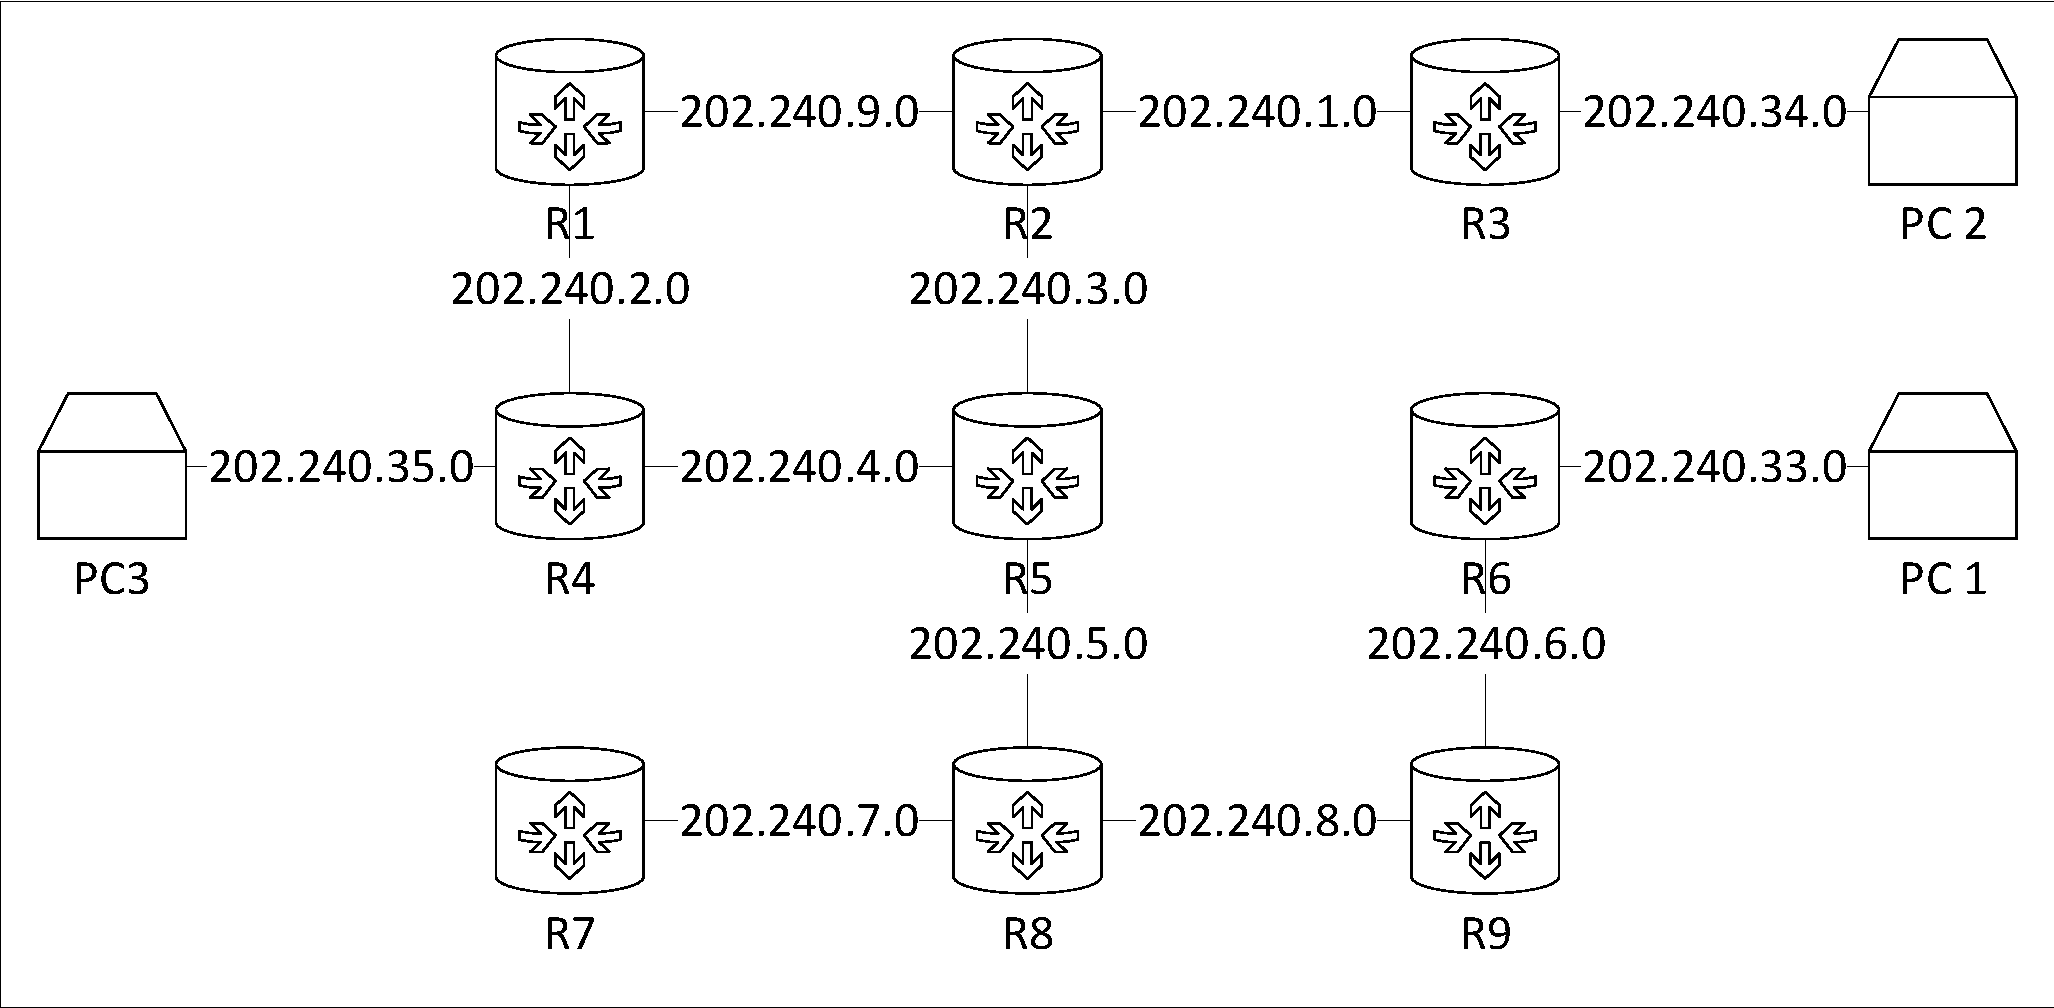
\includegraphics[width=0.9\textwidth]{../data/Lab3.pdf}

共为九台路由器以及三台 PC。
\section{实验目的}

\begin{itemize}
    \item 在上一次实验的基础上实现RIP和OSPF路由协议
    \item 自己设计网络物理拓扑和逻辑网段,并在其上实
    现RIP和OSPF协议
    \item 通过debug信息详细描述RIP和OSPF协议的工作
    过程,包括初始信息交互、路由计算、链路故障处理等部分
    \item RIP协议中观察没有配置水平分割和配置水平分割
    后协议的工作流程,和路由消息传递方式
    \item 观察OSPF中数据库同步信息的格式和同步对象
    以及链路改变信息如何发送
\end{itemize}

\section{实验内容及步骤}

\subsection{启动模拟器}\label{start_emu}
首先将拓扑文件放置在模拟器的 ``net'' 文件夹下,之后编写如下 ``bupt.cmd''
文件作为拓扑文件的启动脚本:

\begin{lstlisting}
@echo off
call bin/script/copyright.cmd
title 控制台,请不要关闭本窗口!
echo * bupt 路由器实验     
echo *====================
cd tmp
"../bin/dynagen/dynagen.exe" ..\net\bupt_3.net
\end{lstlisting}

之后双击 ``0.虚拟服务XP\&2003.bat'' 打开虚拟服务器,确认打开无误后。
再双击打开之前我们编辑的 ``bupt.cmd'',打开控制台。

再打开控制台后,我们就可以根据自己的需要,从列表给出的主机列表中启动一台
或者多台设备准备进行正式的实验。在第一次打开一类机型的设备中的一台的时候,
我们需要为其指定其 ``idlepc'' 值用于后续的匹配,获取 ``idlepc'' 值
并将之保存的指令序列如下(以路由器 R1 为例):

\begin{lstlisting}
idlepc get R1
idlepc save R1 db
\end{lstlisting}

需要注意的是,因为这一款模拟器年久失修,且代码多年无人维护,质量堪忧,我们的
数据可能会在任何时间丢失,因此务必使用好路由器自带的 \texttt{wr} 指令以及
保存好进行配置的指令序列。

\subsection{路由器的配置}

在这次实验中,我们要完成两种协议(RPI 以及 OSPF)的配置。但实际上这两者
的配置方式大同小异,只有在配置协议时才会出现不同,因此在这里我们先简要介绍
下基本的配置流程,然后再介绍两个协议的具体配置方法。

\subsubsection{基本的配置流程}
再保证之前的 ~\ref{start_emu}~ 里面开启的服务没有因为种种原因自动退出后,
我们使用 Windows 系统自带的 \texttt{telnet} 指令连接我们模拟的路由器。

\begin{lstlisting}
telnet 127.0.0.1 <router port specificed by top file>

Connected to Dynamips VM "R1" (ID 0, type c7200) - Console port
Would you like to enter the initial configuration dialog? [yes/no]:
\end{lstlisting}

初次登陆后,路由器的登陆界面会询问我们是否进入初始化的对话。因为我们是要
进行全手动的配置,因此这里选 \texttt{no},之后敲击 \texttt{Enter}
即可进入路由器的 ``Shell'' 界面。

要开始配置路由器,我们需要进入路由器的配置模式,执行如下指令序列:

\begin{lstlisting}
Router>en
Router#conf
Configuring from terminal, memory, or network [terminal]? terminal
Enter configuration commands, one per line.  End with CNTL/Z.
Router(config)#
\end{lstlisting}

在见到 ``Router(config)\#'' 时,就说明我们的路由器进入了配置模式,可以
开始进行配置了。
在路由器上,我们需要配置的内容主要是如下几类:
\begin{itemize}
    \item 打开端口
    \item 在 \texttt{fastEthernet} 口上配置 IP 地址使之能与 PC 机进行通讯
    \item 在 \texttt{serial} 口上配置 IP 地址以及时钟频率,使之能与别的路由器进行通信
    \item 在 \texttt{serial} 口上指定数据链路层的协议为 PPP 协议
\end{itemize}
例如,我们在我们的 \textbf{R3} 上面的配置指令如下:
\begin{lstlisting}
# Config serial interface
interface s 1/0
ip add 202.240.1.2 255.255.255.0
encapsulation PPP
no shutdown
exit
# Config fastEthernet interface
interface f 0/0
ip add 202.240.34.1 255.255.255.0
no shutdown
exit
\end{lstlisting}

\subsubsection{RIP 协议的配置}

在配置 RIP 协议时,我们需要指定的有
\begin{itemize}
    \item 协议的版本
    \item 路由器连接的网段号
    \item 邻居的 IP 地址
\end{itemize}
只有指定了这三个参数,我们的 RIP 协议才可以正确的执行。
例如,在 \textbf{R5} 上我们的配置指令如下:
\begin{lstlisting}
router rip
version 2
network 202.240.3.0
network 202.240.4.0
network 202.240.5.0
neighbor 202.240.3.1
neighbor 202.240.4.1
neighbor 202.240.5.2
exit
\end{lstlisting}

在思科的路由器上,水平分割是默认打开的,
如果我们需要关闭,可以使用 \texttt{no ip split-horizon}
关闭掉。关于 RIP 协议的调试信息可以使用 \texttt{debug ip rip} 看到。
\subsubsection{OSPF 协议的配置}
对于 OSPF 协议,我们不再需要指定邻居的 IP —— 因为 OSPF 协议会自动发现
邻居。但是在配置 OSPF 协议时,我们还额外在路由器之间通信的 \texttt{serial}
口上指定两个延时:其一是发送问候信息的时间间隔,另一个是确认邻居是否还活着的延时。
例如,在我们的 \textbf{R8} 上面配置 OSPF 时候,其指令序列如下:
\begin{lstlisting}
interface s 1/2
clock rate 115200
ip add 202.240.8.1 255.255.255.0
ip ospf hello-interval 5
ip ospf dead-interval 20
encapsulation PPP
no shutdown
exit
router ospf 20
network 202.240.5.0 255.255.255.0 area 0
network 202.240.7.0 255.255.255.0 area 0
network 202.240.8.0 255.255.255.0 area 0
exit
\end{lstlisting}

同样地,我们可以使用 \texttt{debug ip ospf events}、
\texttt{debug ip ospf flood} 以不同的重要程度查看
 OSPF 协议的调试信息。我们还可以使用\texttt{sh ip ospf neighbor}
查看路由器的邻居。

\subsubsection{PC 端的配置流程}
在完成基本的配置流程后,PC 端只需要设置下路由表即可投入使用。我们选择的
策略是将全部的地址都指向 PC 机连接的路由器,\textbf{PC2} 上的配置指令
如下:
\begin{lstlisting}
ip route 0.0.0.0 0.0.0.0 F 0/0
\end{lstlisting}
\section{实验结果}
\subsection{RIP 协议}
\subsubsection{路由表}
在路由器上配置了 RIP 协议后,在很短的时间内即可配置好路由器的路由表。例如,
在全部的路由器上配置了 RIP 协议后,在我们的\textbf{R5} 上面,我们可以
观测到如下的路由表:
\begin{lstlisting}
Router#show ip route
Codes: C - connected, S - static, I - IGRP, R - RIP, M - mobile, B - BGP
       D - EIGRP, EX - EIGRP external, O - OSPF, IA - OSPF inter area
       N1 - OSPF NSSA external type 1, N2 - OSPF NSSA external type 2
       E1 - OSPF external type 1, E2 - OSPF external type 2, E - EGP
       i - IS-IS, su - IS-IS summary, L1 - IS-IS level-1, L2 - IS-IS level-2
       ia - IS-IS inter area, * - candidate default, U - per-user static route
       o - ODR, P - periodic downloaded static route

Gateway of last resort is not set

R    202.240.6.0/24 [120/2] via 202.240.5.2, 00:00:05, Serial1/2
R    202.240.7.0/24 [120/1] via 202.240.5.2, 00:00:05, Serial1/2
     202.240.4.0/24 is variably subnetted, 2 subnets, 2 masks
C       202.240.4.0/24 is directly connected, Serial1/1
C       202.240.4.1/32 is directly connected, Serial1/1
     202.240.5.0/24 is variably subnetted, 2 subnets, 2 masks
C       202.240.5.2/32 is directly connected, Serial1/2
C       202.240.5.0/24 is directly connected, Serial1/2
R    202.240.2.0/24 [120/1] via 202.240.4.1, 00:00:00, Serial1/1
R    202.240.33.0/24 [120/3] via 202.240.5.2, 00:00:05, Serial1/2
     202.240.3.0/24 is variably subnetted, 2 subnets, 2 masks
C       202.240.3.1/32 is directly connected, Serial1/0
C       202.240.3.0/24 is directly connected, Serial1/0
R    202.240.34.0/24 [120/2] via 202.240.3.1, 00:00:08, Serial1/0
R    202.240.1.0/24 [120/1] via 202.240.3.1, 00:00:08, Serial1/0
R    202.240.35.0/24 [120/1] via 202.240.4.1, 00:00:02, Serial1/1
R    202.240.8.0/24 [120/1] via 202.240.5.2, 00:00:08, Serial1/2
R    202.240.9.0/24 [120/1] via 202.240.3.1, 00:00:09, Serial1/0
\end{lstlisting}

通过与我们的拓扑进行对比,不难发现路由表的结果完全正确。

\subsubsection{调试信息}
下面是在 \textbf{R6} 上抓取下来的调试信息:

\begin{lstlisting}
00:35:55: RIP: received v2 update from 202.240.5.1 on Serial1/0
00:35:55:      202.240.1.0/24 via 0.0.0.0 in 2 hops
00:35:55:      202.240.2.0/24 via 0.0.0.0 in 2 hops
00:35:55:      202.240.3.0/24 via 0.0.0.0 in 1 hops
00:35:55:      202.240.4.0/24 via 0.0.0.0 in 1 hops
00:35:55:      202.240.9.0/24 via 0.0.0.0 in 2 hops
00:35:55:      202.240.34.0/24 via 0.0.0.0 in 3 hops
00:35:55:      202.240.35.0/24 via 0.0.0.0 in 2 hops
...
00:36:04: RIP: sending v2 update to 202.240.7.1 via Serial1/1 (202.240.7.2)
00:36:04: RIP: build update entries
00:36:04:       202.240.1.0/24 via 0.0.0.0, metric 3, tag 0
00:36:04:       202.240.2.0/24 via 0.0.0.0, metric 3, tag 0
00:36:04:       202.240.3.0/24 via 0.0.0.0, metric 2, tag 0
00:36:04:       202.240.4.0/24 via 0.0.0.0, metric 2, tag 0
00:36:04:       202.240.5.0/24 via 0.0.0.0, metric 1, tag 0
00:36:04:       202.240.6.0/24 via 0.0.0.0, metric 2, tag 0
00:36:04:       202.240.8.0/24 via 0.0.0.0, metric 1, tag 0
00:36:04:       202.240.9.0/24 via 0.0.0.0, metric 3, tag 0
00:36:04:       202.240.33.0/24 via 0.0.0.0, metric 3, tag 0
00:36:04:       202.240.34.0/24 via 0.0.0.0, metric 4, tag 0
00:36:04:       202.240.35.0/24 via 0.0.0.0, metric 3, tag 0
\end{lstlisting}

在路由器内部,RIP作为一个系统长驻进程而存在于路由器中,
负责从网络系统的其它路由器接收路由信息,从而对本地IP层路由表作动态的维护
,保证IP层发送报文时选择正确的路由。同时负责广播本路由器的路由信息,
通知相邻路由器作相应的修改。

RIP路由协议用“更新(UNPDATES)”和“请求(REQUESTS)”这两种分组来传输信
息的。每个具有RIP协议功能的路由器每隔一定时间给与之直接相连的机
器广播更新信息。更新信息反映了该路由器所有的路由选择信息数据库。路由选择
信息数据库的每个条目由“局域网上能达到的IP地址”和“与该网络的距离”两部分组成
。请求信息用于寻找网络上能发出RIP报文的其他设备。

RIP用“路程段数”(即“跳数”)作为网络距离的尺度。
每个路由器在给相邻路由器发出路由信息时,都会给每个路径加上内部距离。

RIP 的信息格式如图~\ref{fig:RIPHeader}~。

\begin{figure}[!htbp]
    \centering
    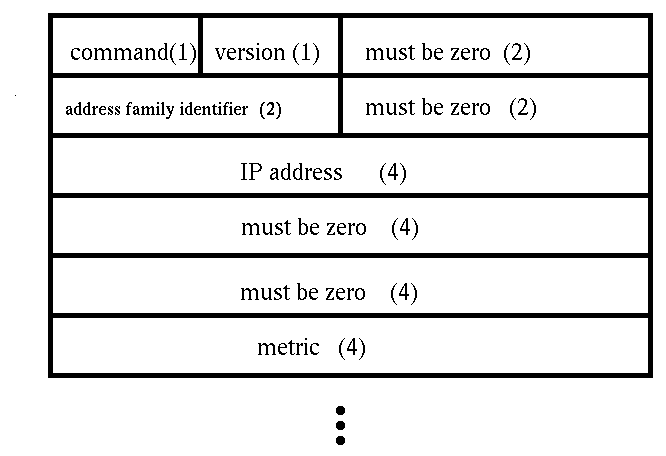
\includegraphics[width=.8\textwidth]{format}
    \caption{RIP Header}
    \label{fig:RIPHeader}
\end{figure}

\subsubsection{路由器不可达对于 RIP 的影响}

RIP 协议的一个缺点就是网络收敛的慢,当一个路由器宕机时,其余路由器到这个
路由器的跳数会一轮一轮的增加到无穷,但实际应用时
我们通常将跳数达到 16 的路由器视为不可达。
尽管后续引入了水平分割以及毒性逆转的方式增快网络收敛
的速度,但是改进后的结果还是不大理想。
在实验中,我们通过关闭 \textbf{R4} 的方式模拟路由器不可达的情况。在经过了一段
较长的时间后,我们在日志中注意到了如下信息:

\begin{lstlisting}
...
00:49:16: RIP: sending v2 update to 202.240.3.1 via Serial1/0 (202.240.3.2)
00:49:16: RIP: build update entries
00:49:16:       202.240.2.0/24 via 0.0.0.0, metric 16, tag 0
00:49:16:       202.240.4.0/24 via 0.0.0.0, metric 16, tag 0
00:49:16:       202.240.5.0/24 via 0.0.0.0, metric 1, tag 0
00:49:16:       202.240.6.0/24 via 0.0.0.0, metric 3, tag 0
00:49:16:       202.240.7.0/24 via 0.0.0.0, metric 2, tag 0
00:49:16:       202.240.8.0/24 via 0.0.0.0, metric 2, tag 0
00:49:16:       202.240.33.0/24 via 0.0.0.0, metric 4, tag 0
00:49:16:       202.240.35.0/24 via 0.0.0.0, metric 16, tag 0
00:49:17: RIP: received v2 update from 202.240.3.1 on Serial1/0
00:49:17:      202.240.2.0/24 via 0.0.0.0 in 16 hops  (inaccessible)
00:49:17:      202.240.4.0/24 via 0.0.0.0 in 16 hops  (inaccessible)
00:49:17:      202.240.35.0/24 via 0.0.0.0 in 16 hops  (inaccessible)
... 
\end{lstlisting}
\subsection{OSPF 协议}
\subsubsection{路由表}
在全部的路由器上配置了 OSPF 协议后,在我们的\textbf{R5} 上面,我们可以
观测到如下的路由表:
\begin{lstlisting}
Router#show ip route
Codes: C - connected, S - static, I - IGRP, R - RIP, M - mobile, B - BGP
       D - EIGRP, EX - EIGRP external, O - OSPF, IA - OSPF inter area
       N1 - OSPF NSSA external type 1, N2 - OSPF NSSA external type 2
       E1 - OSPF external type 1, E2 - OSPF external type 2, E - EGP
       i - IS-IS, su - IS-IS summary, L1 - IS-IS level-1, L2 - IS-IS level-2
       ia - IS-IS inter area, * - candidate default, U - per-user static route
       o - ODR, P - periodic downloaded static route

Gateway of last resort is not set

O    202.240.6.0/24 [110/192] via 202.240.5.2, 00:01:40, Serial1/2
O    202.240.7.0/24 [110/128] via 202.240.5.2, 00:01:40, Serial1/2
     202.240.4.0/24 is variably subnetted, 2 subnets, 2 masks
C       202.240.4.0/24 is directly connected, Serial1/1
C       202.240.4.1/32 is directly connected, Serial1/1
     202.240.5.0/24 is variably subnetted, 2 subnets, 2 masks
C       202.240.5.2/32 is directly connected, Serial1/2
C       202.240.5.0/24 is directly connected, Serial1/2
O    202.240.2.0/24 [110/128] via 202.240.4.1, 00:01:40, Serial1/1
O    202.240.33.0/24 [110/193] via 202.240.5.2, 00:01:40, Serial1/2
     202.240.3.0/24 is variably subnetted, 2 subnets, 2 masks
C       202.240.3.1/32 is directly connected, Serial1/0
C       202.240.3.0/24 is directly connected, Serial1/0
O    202.240.34.0/24 [110/129] via 202.240.3.1, 00:01:46, Serial1/0
O    202.240.1.0/24 [110/128] via 202.240.3.1, 00:01:47, Serial1/0
O    202.240.35.0/24 [110/65] via 202.240.4.1, 00:01:47, Serial1/1
O    202.240.8.0/24 [110/128] via 202.240.5.2, 00:01:47, Serial1/2
O    202.240.9.0/24 [110/128] via 202.240.3.1, 00:01:47, Serial1/0
\end{lstlisting}

\subsubsection{调试信息}
\begin{lstlisting}
00:07:48: OSPF: Rcv hello from 202.240.35.1 area 0 from Serial1/1 202.240.4.1
00:07:48: OSPF: End of hello processing
00:07:52: OSPF: Rcv hello from 202.240.9.2 area 0 from Serial1/0 202.240.3.1
00:07:52: OSPF: End of hello processing
00:07:53: OSPF: Rcv hello from 202.240.35.1 area 0 from Serial1/1 202.240.4.1
00:07:53: OSPF: End of hello processing
00:07:55: OSPF: Rcv hello from 202.240.8.1 area 0 from Serial1/2 202.240.5.2
00:07:55: OSPF: Interface Serial1/2 going Up
00:07:56: %LINEPROTO-5-UPDOWN: Line protocol on Interface Serial1/2, changed state to up
00:07:57: OSPF: Rcv hello from 202.240.9.2 area 0 from Serial1/0 202.240.3.1
00:07:57: OSPF: End of hello processing
00:07:58: OSPF: Rcv hello from 202.240.35.1 area 0 from Serial1/1 202.240.4.1
00:07:58: OSPF: End of hello processing
00:08:00: OSPF: Rcv hello from 202.240.8.1 area 0 from Serial1/2 202.240.5.2
00:08:00: OSPF: 2 Way Communication to 202.240.8.1 on Serial1/2, state 2WAY
00:08:00: OSPF: Send DBD to 202.240.8.1 on Serial1/2 seq 0x1004 opt 0x42 flag 0x7 len 32
00:08:00: OSPF: End of hello processing
00:08:00: OSPF: Rcv DBD from 202.240.8.1 on Serial1/2 seq 0x9C5 opt 0x42 flag 0x7 len 32  mtu 1500 state EXSTART
00:08:00: OSPF: NBR Negotiation Done. We are the SLAVE
00:08:00: OSPF: Send DBD to 202.240.8.1 on Serial1/2 seq 0x9C5 opt 0x42 flag 0x2 len 132
00:08:01: OSPF: Rcv DBD from 202.240.8.1 on Serial1/2 seq 0x9C6 opt 0x42 flag 0x3 len 52  mtu 1500 state EXCHANGE
00:08:01: OSPF: Send DBD to 202.240.8.1 on Serial1/2 seq 0x9C6 opt 0x42 flag 0x0 len 32
00:08:01: OSPF: Database request to 202.240.8.1
00:08:01: OSPF: sent LS REQ packet to 202.240.5.2, length 12
00:08:01: OSPF: Rcv DBD from 202.240.8.1 on Serial1/2 seq 0x9C7 opt 0x42 flag 0x1 len 32  mtu 1500 state EXCHANGE
00:08:01: OSPF: Exchange Done with 202.240.8.1 on Serial1/2
00:08:01: OSPF: Send DBD to 202.240.8.1 on Serial1/2 seq 0x9C7 opt 0x42 flag 0x0 len 32
00:08:01: OSPF: Synchronized with 202.240.8.1 on Serial1/2, state FULL
00:08:01: %OSPF-5-ADJCHG: Process 20, Nbr 202.240.8.1 on Serial1/2 from LOADING to FULL, Loading Done
00:08:02: OSPF: Rcv hello from 202.240.9.2 area 0 from Serial1/0 202.240.3.1
00:08:02: OSPF: End of hello processing
\end{lstlisting}

在这份调试信息上,我们可以清晰的看到 OSPF 的 Hello 包发送以及互相交换数据库的详细信息。
其符合 OSPF 的特点。

OSPF 的包头如下:

\begin{lstlisting}
0                   1                   2                   3
0 1 2 3 4 5 6 7 8 9 0 1 2 3 4 5 6 7 8 9 0 1 2 3 4 5 6 7 8 9 0 1
+-+-+-+-+-+-+-+-+-+-+-+-+-+-+-+-+-+-+-+-+-+-+-+-+-+-+-+-+-+-+-+-+
|   Version #   |     Type      |         Packet length         |
+-+-+-+-+-+-+-+-+-+-+-+-+-+-+-+-+-+-+-+-+-+-+-+-+-+-+-+-+-+-+-+-+
|                          Router ID                            |
+-+-+-+-+-+-+-+-+-+-+-+-+-+-+-+-+-+-+-+-+-+-+-+-+-+-+-+-+-+-+-+-+
|                           Area ID                             |
+-+-+-+-+-+-+-+-+-+-+-+-+-+-+-+-+-+-+-+-+-+-+-+-+-+-+-+-+-+-+-+-+
|           Checksum            |             AuType            |
+-+-+-+-+-+-+-+-+-+-+-+-+-+-+-+-+-+-+-+-+-+-+-+-+-+-+-+-+-+-+-+-+
|                       Authentication                          |
+-+-+-+-+-+-+-+-+-+-+-+-+-+-+-+-+-+-+-+-+-+-+-+-+-+-+-+-+-+-+-+-+
|                       Authentication                          |
+-+-+-+-+-+-+-+-+-+-+-+-+-+-+-+-+-+-+-+-+-+-+-+-+-+-+-+-+-+-+-+-+
\end{lstlisting}

至于各个包的详细格式,还请参阅 https://www.freesoft.org/CIE/RFC/1583/99.htm

\subsubsection{路由器不可达对于 OSPF 的影响}
当我们关闭 \textbf{R2} 时,在 \textbf{R5} 上可以看到如下信息:
\begin{lstlisting}
00:22:45: OSPF: End of hello processing
00:22:50: OSPF: Rcv hello from 202.240.8.1 area 0 from Serial1/2 202.240.5.2
00:22:50: OSPF: End of hello processing
00:22:55: OSPF: Rcv hello from 202.240.8.1 area 0 from Serial1/2 202.240.5.2
00:22:55: OSPF: End of hello processing
00:22:57: OSPF: 202.240.9.2 address 202.240.3.1 on Serial1/0 is dead
00:22:57: %OSPF-5-ADJCHG: Process 20, Nbr 202.240.9.2 on Serial1/0 from FULL to DOWN, Neighbor Down: Dead timer expired
00:22:57: Inc retrans unit nbr count index 3 (0/3) to 1/1
00:22:57: Set Nbr 202.240.8.1 3 first flood info from 0 (0) to 624D627C (22)
00:22:57: Init Nbr 202.240.8.1 3 next flood info to 624D627C
00:22:57: OSPF: Add Type 1 LSA ID 202.240.5.1 Adv rtr 202.240.5.1 Seq 80000008 to Serial1/2 202.240.8.1 retransmission list
00:22:57: OSPF: Start Serial1/2 202.240.8.1 retrans timer
00:22:57: Set idb next flood info from 0 (0) to 624D627C (22)
00:22:57: OSPF: Add Type 1 LSA ID 202.240.5.1 Adv rtr 202.240.5.1 Seq 80000008 to Serial1/2 flood list
00:22:57: OSPF: Start Serial1/2 pacing timer
00:22:57: OSPF: Build router LSA for area 0, router ID 202.240.5.1, seq 0x80000008
00:22:57: OSPF: Flooding update on Serial1/2 to 224.0.0.5 Area 0
00:22:57: OSPF: Send Type 1, LSID 202.240.5.1, Adv rtr 202.240.5.1, age 1, seq 0x80000008 (0)
00:22:57: Create retrans unit 0x626F4864/0x624D4EDC 3 (0/3) 1
00:22:57: OSPF: Set nbr 3 (0/3) retrans to 4788 count to 0
00:22:57: Set idb next flood info from 624D627C (22) to 0 (0)
00:22:57: OSPF: Remove Type 1 LSA ID 202.240.5.1 Adv rtr 202.240.5.1 Seq 80000008 from Serial1/2 flood list
00:22:57: OSPF: Stop Serial1/2 flood timer
00:23:00: OSPF: Received ACK from 202.240.8.1 on Serial1/2
00:23:00: OSPF: Rcv Ack Type 1, LSID 202.240.5.1, Adv rtr 202.240.5.1, age 1, seq 0x80000008
00:23:00: Dec retrans unit nbr count index 3 (0/3) to 0/0
00:23:00: Free nbr retrans unit 0x626F4864/0x624D4EDC 0 total 0. Also Free nbr retrans block
00:23:00: Set Nbr 202.240.8.1 3 first flood info from 624D627C (22) to 0 (0)
00:23:00: Adjust Nbr 202.240.8.1 3 next flood info to 0
00:23:00: OSPF: Remove Type 1 LSA ID 202.240.5.1 Adv rtr 202.240.5.1 Seq 80000008 from 202.240.8.1 retransmission list
00:23:00: OSPF: Stop nbr 202.240.8.1 retransmission timer
00:23:00: OSPF: Rcv hello from 202.240.8.1 area 0 from Serial1/2 202.240.5.2
00:23:00: OSPF: End of hello processing
\end{lstlisting}

可以看到,在关闭 R2 后,R5 很快就发现 R2 挂掉了,并向其他的路由器发送了同步信息。
\section{实验中的问题及心得}

在实验中,除了遇到了很多次 Dynimips 无理取闹式的崩溃之外,十分顺利,并没有
遇到任何的问题。这要感谢老师认真准备的 PPT,简明扼要的给我们指出了
如何使用路由器的指令完成实验。

至于心得,就是无论何时都要有足够的备份,否则无法从容面对随时都会崩溃的软件
还要完成实验。

%\color{white}再就是,垃圾助教NM$L。

\section{实验思考}
\subsection{实验中,采用下一跳和转发接口这两种方式配置PC2和PC3有什么区别?
会导致在你的拓扑结构中丢包数有什么变化?用arp表中的内容来解释}
PC 2 ping PC 3。
\begin{lstlisting}
Router#show arp
Protocol  Address          Age (min)  Hardware Addr   Type   Interface
Internet  202.240.35.1            0   ca02.2a20.0000  ARPA   FastEthernet0/0
Internet  202.240.35.2            0   ca02.2a20.0000  ARPA   FastEthernet0/0
Internet  202.240.34.33           -   c80a.2a20.0000  ARPA   FastEthernet0/0
Internet  202.240.2.1             2   ca02.2a20.0000  ARPA   FastEthernet0/0
Router#ping 202.240.35.33

Type escape sequence to abort.
Sending 5, 100-byte ICMP Echos to 202.240.35.33, timeout is 2 seconds:
..!!!
Success rate is 60 percent (3/5), round-trip min/avg/max = 364/425/460 ms
Router#show arp
Protocol  Address          Age (min)  Hardware Addr   Type   Interface
Internet  202.240.35.1            0   ca02.2a20.0000  ARPA   FastEthernet0/0
Internet  202.240.35.2            0   ca02.2a20.0000  ARPA   FastEthernet0/0
Internet  202.240.35.33           0   ca02.2a20.0000  ARPA   FastEthernet0/0
Internet  202.240.34.33           -   c80a.2a20.0000  ARPA   FastEthernet0/0
Internet  202.240.2.1             2   ca02.2a20.0000  ARPA   FastEthernet0/0
\end{lstlisting}

PPP链路网络中使用转发接口,不需要进行 ARP 解析即可发送数据。
以太网则需要进行ARP解析,每次解析都会发生丢包。
\subsection{对照所截获的消息,解释OSPF协议在邻居发现、
链路状态数据库同步和链路状态更新时每条消息的含义}
见第四章。

\subsection{写出在你的拓扑中,数据包从某台PC发送给同一网络中
的PC和不同网络中的PC的完整过程}
在 \texttt{ping} 命令之前, PC3 的 arp 表只有自己的 f0/0 端口的 MAC 地址,R4 只有
自己 f0/0 口的 MAC 地址,R1、R2 的 arp 表为空, R3的 arp 表只有自己的 f0/0 端口的
MAC 地址,PC2 的 arp 表只有自己的 f0/0 端口的 MAC 地址。ping PC3 的时候,PC2会把包发向默认路由器
,但是 PC2 并不知道 PC3 的 MAC 地址,而链路层一定是要 MA 来寻址。
所以 PC2 会发一个包询问 PC3 的 MAC 地址,这是丢失的第一个包。
然后数据包在路由器见转移到了 R4 后,同样不知道 PC3 的 MAC 地址,
需要发送一个包询问 PC4 的 MAC 
地址,这是丢失的第二个包。之后的 \texttt{ping} 都会成功。
\end{document}